\documentclass[22pt]{beamer}
% \documentclass[handout]{beamer}
% add theme and color theme https://www.overleaf.com/learn/latex/Beamer#Reference_guide
\setbeamertemplate{navigation symbols}{} % hides navigation buttons
\setbeamertemplate{footline}[frame number]
\usepackage[utf8]{inputenc}
\usepackage{minted}
\usepackage{graphicx}
\usepackage[absolute,overlay]{textpos}
\usepackage{comment}
\usepackage{color}
\usepackage{xcolor}
\usepackage{hyperref}
\usepackage{enumitem}
\setlist[itemize]{label=\textbullet, labelsep=1em, leftmargin=2em}
\usepackage{caption}


\newcommand{\code}[1]{\colorbox{gray!10}{\texttt{#1}}}
\newcommand{\desclabel}[1]{\textcolor{cyan}{#1}}
\newcommand{\codeTour}{
    \begin{textblock*}{1.3cm}(11cm,0.5cm) % {block width}(xcoord, ycoord)
    
\includegraphics[width=1.3cm]{Bilder/CodeTour.png}
    \end{textblock*}
}
\newcommand{\terminal}{
    \begin{textblock*}{1.3cm}(11cm,0.5cm) % {block width}(xcoord, ycoord)
    
\includegraphics[width=1.3cm]{Bilder/terminal.png}
    \end{textblock*}
}

\usemintedstyle{tango}
\pagenumbering{roman}

\title{Docker something}
\author{Julia Winkler}
\date{19.06.2024}

\begin{document}

%% TODO: layout element, dass kennzeichnet, wann man ins terminal wechselt vgl. "Vorlesung" bei EAE
%% TODO: how to make one list item without overhead -> macro?
%% einheitliche Sprache

\begin{frame}[plain]
    \vfill
    \begin{center}
        
\includegraphics[width=1\textwidth]{Bilder/docker-how.png}
    \end{center}
    \vfill
\end{frame}

\maketitle

\begin{frame}[plain]
    \frametitle{Gliederung}
    \tableofcontents
\end{frame}

\subsection{Einführung}
\begin{frame}
    \frametitle{Wiso, Weshalb, Warum?}
    \begin{center}
        
\includegraphics[width=0.8\textwidth]{Bilder/docker-why.png}
    \end{center}\pause
    \begin{center}
        "a sandboxed process on your machine that is isolated from all other processes on the host machine"
    \end{center}\pause
    \begin{center}
        "It works on my computer"
    \end{center}\pause
    \begin{center}
        "faster onboarding and testing while also simplifying the deployment of services"
    \end{center}
\end{frame}

\begin{frame}[t]
    \frametitle{Wer ist Moby Dock?}\pause
    \only<2>{\begin{figure}[h]
        \centering
        
\includegraphics[width=0.8\textwidth]{Bilder/mobydocker.jpg}
    \end{figure}
    }
    \only<3>{\begin{figure}[h]
        \centering
        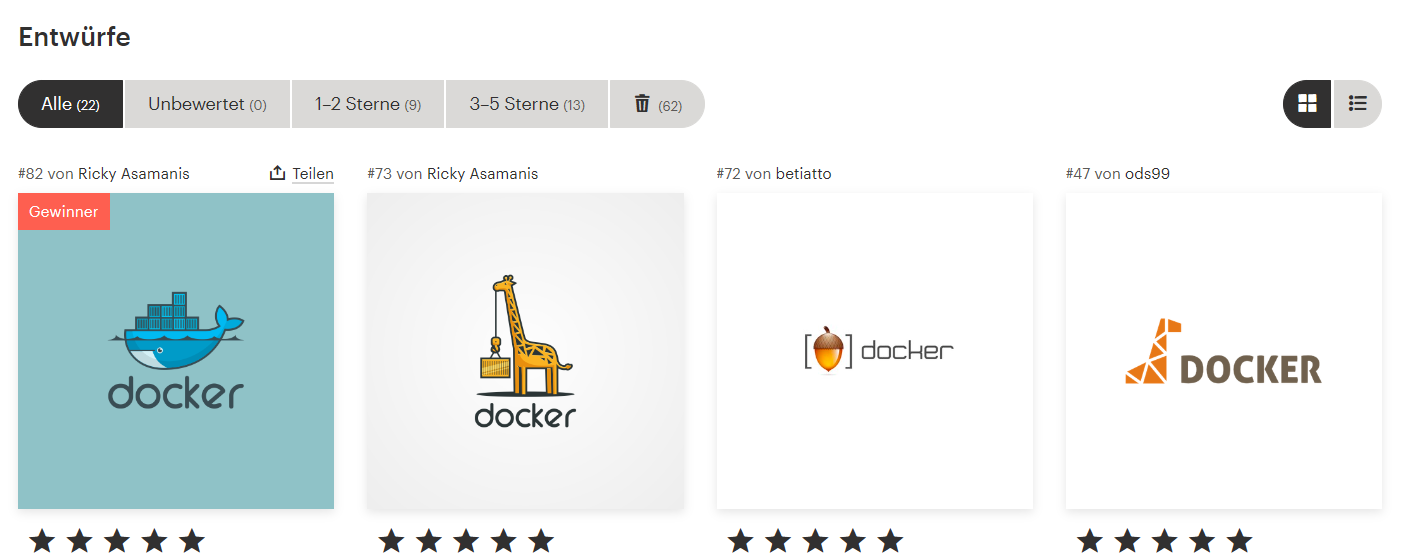
\includegraphics[width=0.95\textwidth]{Bilder/wettbewerb.png}
        \caption*{Wettbewerb zum Icon für Docker}
    \end{figure}
    }
\end{frame}

\begin{frame}[t]
    \frametitle{Was ist Docker?}
    \begin{block}{Docker}
        freie Software zur Isolierung von Anwendungen\newline
        Containervirtualisierung\newline
        "light weight" Virtual Maschine\newline
    \end{block}
    \begin{figure}[h]
        \centering
        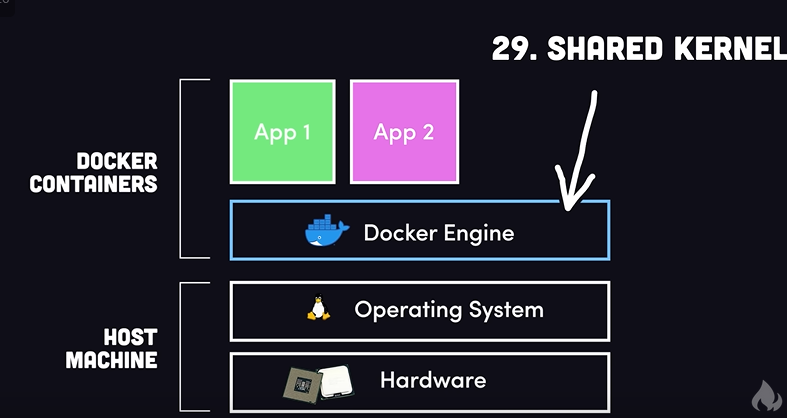
\includegraphics[width=0.9\textwidth]{Bilder/Docker Concept.png}
    \end{figure}
\end{frame}


\begin{frame}[t]
    \frametitle{Wichtige Begriffe}
    
    \begin{block}{Container}
        Umgebung in der die tatsächliche Anwendung läuft
    \end{block}
    \begin{block}{Image}
        Blaupausen, um einen Container zu erstellen
    \end{block}
    \begin{block}{Dockerfile}
        Anleitung, um ein Image zu erstellen
    \end{block}
    \begin{block}{Registry}
        z.B. Docker Hub, EAC....
        Ort an dem viele verschindene Images gespeichert und geteilt werden können
    \end{block}
    \begin{block}{Docker Compose}
        Orchestrierungstool für Dockerfile\newline
        Wrapper für einen oder mehrere Container
    \end{block}
    %%\begin{block}{Docker Desktop}
    %%    - UI für alles was man in der CLI machen kann (?) %% TODO: 
    %%\end{block}
\end{frame}

\begin{frame}[c]
    \frametitle{Zusammenhang der Docker Komponenten}
        \includegraphics<1>[width=1\textwidth]{Bilder/Docker-Ablauf.png}
        \includegraphics<2>[width=1\textwidth]{Bilder/dockercommand.png}
\end{frame}

\begin{frame}[t]
    \frametitle{Wie kreige ich dieses "Docker"?}
    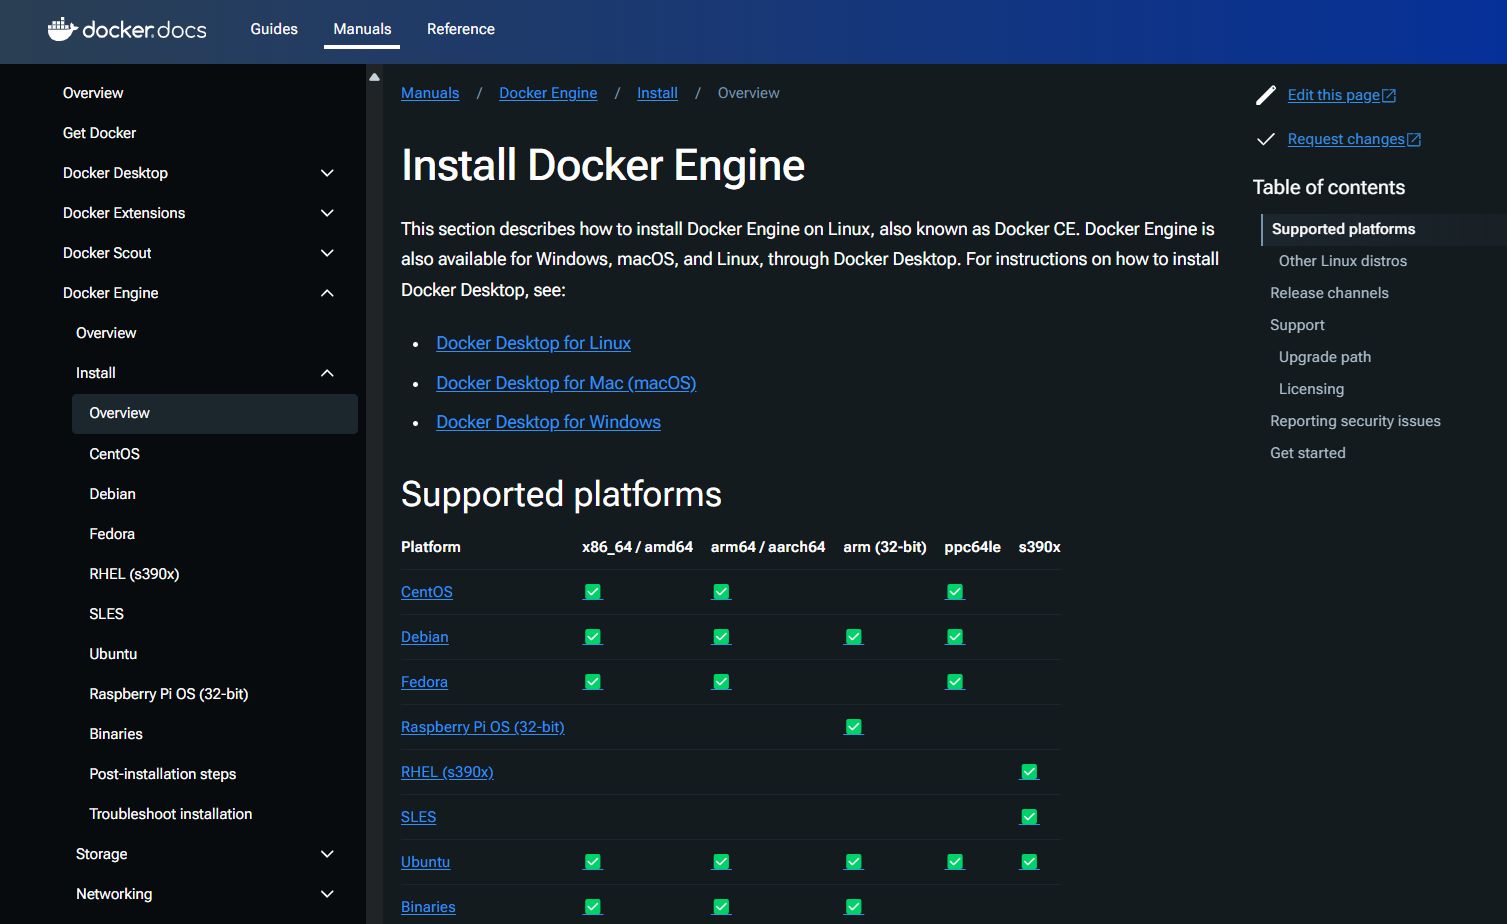
\includegraphics[width=0.9\textwidth]{Bilder/Installation.png}

    \href{https://docs.docker.com/engine/install}{Doku}
\end{frame}

\begin{frame}[fragile]
    \frametitle{Hello World}
    \terminal
    \begin{minted}{bash}
    > docker -v
    > docker --help
    > docker run hello-world
    \end{minted}
\end{frame}

\subsection{Dockerfile}
\begin{frame}[c]
    \frametitle{Zusammenhang der Docker Komponenten}
    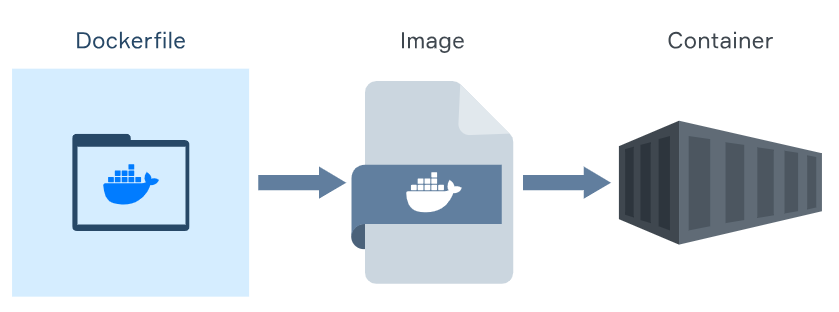
\includegraphics[width=1\textwidth]{Bilder/Docker-Ablauf_dark.png}
\end{frame}

\begin{frame}[fragile]
    \frametitle{Dockerfile}
    \begin{itemize}
        \item Ein Dockerfile ist die Anleitung um ein Image zu erstellen.
        %% Mit einem Dockerfile kann man den Inhalt des Containers configurieren
        \item Standardmäßig hießt die Datei 'Dockerfile'
        \item wieter Optionen mit \code{docker buildx build}
    \end{itemize}
    \begin{figure}[h]
        \centering
        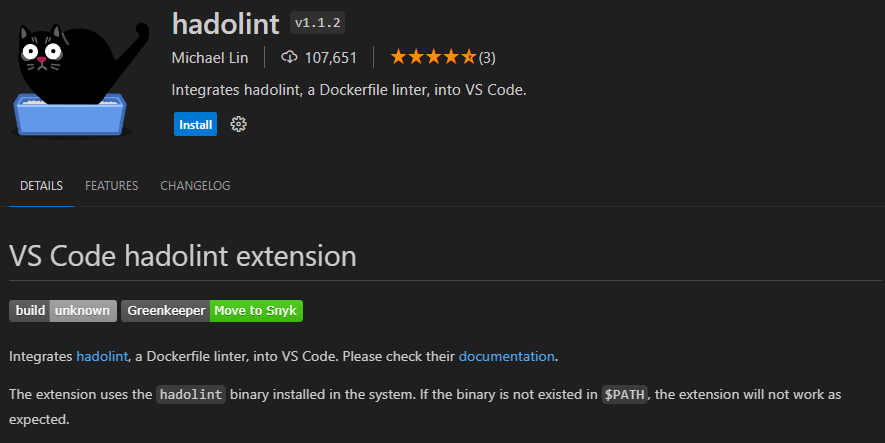
\includegraphics[width=0.6\textwidth]{Bilder/Hadolint.png}
        \caption*{Plugin für die Arbeit mit Docker}
    \end{figure}

\end{frame}

\begin{frame}[fragile]
    \frametitle{docker build command}
    \code{docker build [OPTIONS] PATH | URL | -} 
    
    \-  \ Build an image from a Dockerfile

    \code{[OPTIONS]}
    \begin{description}[labelindent=0.5cm, style=unboxed, labelwidth=\widthof{-f, --file string}, leftmargin=!]
        \item[\desclabel{-f, --file string}] Name of the Dockerfile (default: "PATH/Dockerfile")
        \item[\desclabel{-t, --tag stringArray}] Name and optionally a tag (format: "name:tag")
        \item[\desclabel{PATH}] in most cases .
    \end{description}

    Beispiele: %% TODO: test commands
    \begin{minted}[fontsize=\small]{bash}
    docker build . # 'Dockerfile' im aktuellen Ordner
    docker build -t myimage:v1 . 
    docker build -f Docker.cmd . 
    docker build ./examples/FastAPI/Dockerfile
    \end{minted}
    
\end{frame}

%% Ü: Wie sieht also ein Dockerfile aus
\begin{frame}[fragile]
    \frametitle{Dockerfile}
    \codeTour

    Beispiel \code{Dockerfile}: 
    \inputminted[fontsize=\footnotesize, frame=lines]{Dockerfile}{../examples/Dockerfile}\medskip 
    Weitere Informationen und Instruction
    \href{https://docs.docker.com/reference/dockerfile/#overview}{https://docs.docker.com/reference/dockerfile/}
\end{frame}

\begin{frame}[fragile]
    \frametitle{CMD vs. ENTRYPOINT}
    \terminal
    \begin{minted}{bash}
    > docker build -t example:cmd -f Dockerfile.cmd .
    > docker build -t example:entry -f Dockerfile.entry .
    \end{minted} 
    \pause
    \begin{minted}{bash}
    > docker run example:cmd
    > docker run example:cmd hello
    > docker run example:entry hello        
    \end{minted}
    \pause \medskip
    \begin{itemize}
        \item beide definieren den, was nach Container start ausgeführt wird
        \item \code{CMD} kann überschrieben werden
        \item \code{ENTRYPOINT} bestimmt den command, neue Parameter werden angehangen
    \end{itemize}
\end{frame}

\begin{frame}[fragile]
    \frametitle{RUN} %% TODO: Dockerfiles hier mit einbinden??
    \begin{minted}{bash}
    > docker build -t example:single -f Dockerfile.single .
    > docker build -t example:multi -f Dockerfile.multi .

    # Entstandene Images anschauen
    > docker ps -a
    > docker images
    \end{minted}
    \pause\medskip
    \begin{itemize}
        \item pro \code{RUN} baut Docker einen Layer
        \item Layer werden gecached und nach Möglichkeit wiederverwendet
        \item versucht \code{RUN} instructions zu verbinden
        \item verbessert built-time und Image größe
    \end{itemize}
\end{frame}
%% vllt Docker mit ubuntu for exec, it, start, stop, name

\begin{frame}[fragile]
    \frametitle{Python bsp}
    \inputminted[fontsize=\footnotesize, frame=lines]{dockerfile}{../examples/Dockerfile.cmd}
    %% run mit volume und port
    %% start, stop, rm
\end{frame}

\begin{frame}[t]
    \frametitle{Volumes}
    \begin{itemize}
        \item 
    \end{itemize} 
\end{frame}

\begin{frame}[fragile]
    \frametitle{React}
    \inputminted[fontsize=\footnotesize, frame=lines]{dockerfile}{../examples/Dockerfile.cmd}
\end{frame}

\begin{frame}[t]
    \frametitle{Multistage builds}
    \begin{itemize}
        \item 1
    \end{itemize} 
\end{frame}

\begin{frame}[fragile]
    \frametitle{React - Multistage}
    \inputminted[fontsize=\footnotesize, frame=lines]{dockerfile}{../examples/Dockerfile.cmd}
\end{frame}

\begin{frame}[t]
    \frametitle{Dockerfile Best practices}
    \begin{itemize}
        \item RUN commands
        \item Order of COPY
        \item Volumes
        \item Multistage
    \end{itemize} 
\end{frame}

\begin{frame}[t]
    \frametitle{Docker Compose}
    \begin{itemize}
        \item Vorteile
        \item UseCases
    \end{itemize} 
\end{frame}

\begin{frame}[fragile]
    \frametitle{Docker Compose zu Python}
    \inputminted[fontsize=\footnotesize, frame=lines]{dockerfile}{../examples/Dockerfile.cmd}
\end{frame}

\begin{frame}[fragile]
    \frametitle{Docker Compose Webapp}
    \inputminted[fontsize=\footnotesize, frame=lines]{dockerfile}{../examples/Dockerfile.cmd}
\end{frame}

\begin{frame}[t]
    \frametitle{title}
    \begin{itemize}
        \item OpenDrone Map
        \item [Nathalies Kubernetes Arbeit]
        \item [Felix Hiwi arbeit]
        \item [deply your app on a cloud hosted frame work]
    \end{itemize}
\end{frame}

\begin{frame}[t]
    \frametitle{Cheatsheet}
    \begin{itemize}
        \item docker run
        \item docker build
        \item docker push, pull
        \item docker ps -a
        \item docker rm / rmi
        \item ...
    \end{itemize} 
\end{frame}

\begin{frame}[t]
    \frametitle{Coole Quellen und so weiter}
    \begin{itemize}
        \item \href{https://www.docker.com/}{https://www.docker.com/}
        \item \href{https://docs.docker.com/get-started/}{https://docs.docker.com/get-started/}
        \item 
    \end{itemize} 
\end{frame}

\begin{comment}

\begin{frame}[t]
    \frametitle{title}
    \begin{itemize}
        \item 1
    \end{itemize} 
\end{frame}

\begin{frame}[fragile]
    \frametitle{title}
    \inputminted[fontsize=\footnotesize, frame=lines]{dockerfile}{../examples/Dockerfile.cmd}
\end{frame}

\begin{wrapfigure}{l}{0.25\textwidth}
    \centering
    \includegraphics[width=0.25\textwidth]{contour}
\end{wrapfigure}

\begin{figure}[h]
    \centering
    \includegraphics[width=0.5\textwidth]{spiral}
    \caption{}
\end{figure}
    
\end{comment}

\end{document}